% !TEX encoding = UTF-8 Unicode
%!TEX root = main.tex
% !TEX spellcheck = en-US
%%=========================================


%%%%%%%%%%%%%%%%%%%%%%%%%%%%%%%%%%%%%%%%%%%%%%%%%%%%%%%%%%%%%%%%%%%%%%%%%%%%%%%%%%%
\chapter{Design and Implementation}
\label{ch:design_implementation}
% each feature/

This chapter describes in detail the design and implementation of ProXC++. This includes the runtime data structures used by the scheduler, and how the library features interact with the scheduler and the runtime environment.

Note that the focus of this design and implementation is dynamic multithreading and multicore support. Features and details that has not much relevance to multithreading, such as replicators and C++ syntax, is detailed to a lesser extent.

The library is written in C++, with standard C++14 dialect. The reader is expected to have a fair understanding of C++, and being familiar with standard C++11 dialect is recommended. Detailed explanations of the C++ programming language is not presented here. Refer to any C++ reference (e.g. \citet{stroustrup2013c++}) for more details.


%%%%%%%%%%%%%%%%%%%%%%%%%%%%%%%%%%%%%%%%%%%%%%%%%%%%%%%%%%%%%%%%%%%%%%%%%%%%%%%%
\section{Data Structures}
% intrusive queues/sets
% spinlocks


\FloatBarrier
%%%%%%%%%%%%%%%%%%%%%%%%%%%%%%%%%%%%%%%%%%%%%%%%%%%%%%%%%%%%%%%%%%%%%%%%%%%%%%%%
\section{Runtime System Overview}
\label{sec:runtime_system_overview}

The runtime system for ProXC++ is based on \textit{contexts}, which represent a point of computational execution. A context is a user\hyp{}thread, meaning it has its own program stack and processor context. A kernel\hyp{}thread always has a main context and a scheduler context, while it may have zero or more work contexts. Contexts are based on the hybrid threading model (see \cref{subsec:threading_models}).

At startup, the initial main context creates $N-1$ kernel\hyp{}threads, given the processor has $N$ online logical cores. Each main context then creates a scheduler context, which represent the runtime environment for each kernel\hyp{}thread. Only the initial main context does any meaningful work, as the other main contexts only purpose is to spawn and join the scheduler context. Whenever the initial main context returns, the runtime environment will cleanup and shutdown. At the creation of a new kernel\hyp{}thread, along side with its main context and scheduler context, the scheduler will wait as idle (block) until available work is ready in other schedulers.

\Cref{fig:runtime_overview} displays a rough outline of how the contexts, user\hyp{}threads and kernel\hyp{}threads are organized relative to each other. Note that even though work contexts are present in each kernel\hyp{}thread, it 

\begin{figure}[h!]
    \centering
    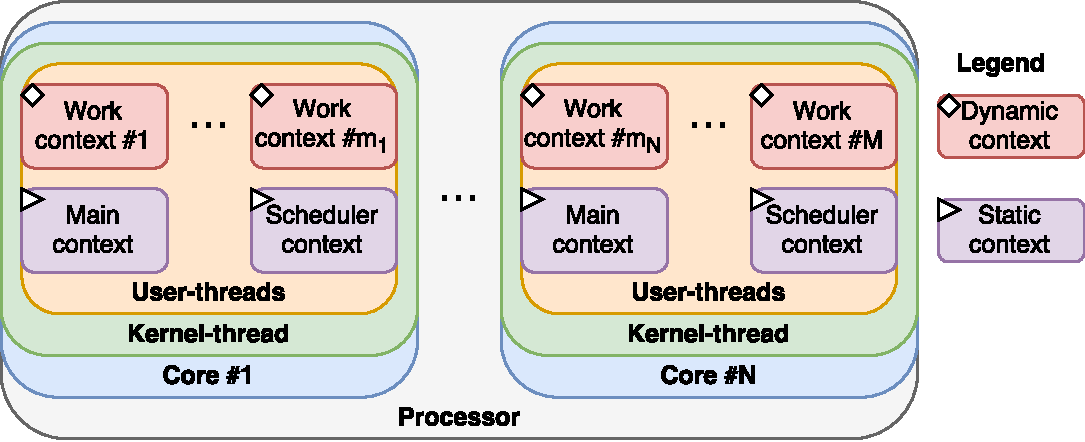
\includegraphics[width=0.8\linewidth]{fig/runtime_overview}
    \caption{Overview of the runtime system, with N online processor cores.}
    \label{fig:runtime_overview}
\end{figure}

Work is distributed among schedulers through work stealing (see \cref{subsec:work_stealing}). This is achieved by each scheduler having a double\hyp{}ended queue (deque for short) containing ready work for that given scheduler. Whenever work is spawned by a scheduler, or idle work becomes ready, it is pushed onto the deque. This allows idle schedulers to try steal work and resume.


\FloatBarrier
%%%%%%%%%%%%%%%%%%%%%%%%%%%%%%%%%%%%%%%%%%%%%%%%%%%%%%%%%%%%%%%%%%%%%%%%%%%%%%%%
\section{Contexts}
\label{sec:contexts}

The runtime system differentiates contexts in two categories: \textit{process vs. scheduler} and \textit{static vs. dynamic}.

A process context represents a part of computation from the program, while the scheduler context is, as the name implies, the scheduler which is in control of scheduling the different process contexts. A static context is a context which cannot \textit{migrate} between schedulers, while a dynamic context can.

For every kernel\hyp{}thread, there always exist a \textit{main context} and a \textit{scheduler context}. The main context is the context of the actual kernel\hyp{}thread, meaning the kernel\hyp{}thread returns when the main context returns. It is a process context, since it represents a part of the computation in the program, and a static context, since it cannot migrate between schedulers. It is undefined behaviour FIXME for main context to return (exit) on a kernel\hyp{}thread different from where it originated from, which is why the main context is static.

The scheduler context is responsible for creating new work contexts, schedule between work contexts, and destroying finished work contexts. The scheduler is never visible to the programmer, and is the driving force behind the runtime environment. The scheduler is obviously a static context, as having multiple schedulers on the same kernel\hyp{}thread is unintuitive and unproductive.

Besides the main and scheduler context, the rest of the program is composed by \textit{work contexts}. Work contexts are process contexts, but opposed to the main context, are dynamic instead of static. Being dynamic allows work contexts to migrate between schedulers. 

Contexts are implemented using the Boost Context library \citep{kowalke2017boost}. Boost Context creates an abstraction over the execution state of a thread called \textit{execution context}, which includes stack and stack pointer, local variables, CPU registers and flags, and instruction pointer. The execution context allows transfer of control between other execution contexts, allowing to build higher level abstractions such as user\hyp{}threads.

The context data structure is represented as a class, containing an execution context as well as a collection of flags, \textit{intrusive hooks}\footnote{Data members stored in the class object itself used by intrusive containers to insert the class object into the container}, a wait queue, and a spinlock. The context class only acts as an information container for a given user\hyp{}thread, as most of the functionality of the context is implemented by the scheduler.


%%%%%%%%%%%%%%%%%%%%%%%%%%%%%%%%%%%%%%%%%%%%%%%%%%%%%%%%%%%%%%%%%%%%%%%%%%%%%%%%
\section{Scheduler}

% work stealing
% process create, schedule, join, destroy
% process timeouts

\section{Parallel}


\section{Timers}


\section{Channels}

\section{Alt}

